\subsection{Classification trees}

The following section has the purpose to use tree-based classification methods to find a model which will predict if an NBA's rookie career will be longer than five years.

We started to analyze the data through classification trees using the \textit{gini} minimization function. The result is a complex tree which is difficult to read (109 terminal nodes).

To understand whether it was better to use a simpler tree or not, we performed cross-validation using different levels of tree size and evaluated the impact on the test error.

\Fig~\ref{fig:tree_cv_plot} shows the trends of the deviance and the penalization factor \textit{k} for different values of tree size as determined by cross-validation. In \Fig~\ref{fig:trees_size} are shown the obtained trees with different sizes.

\begin{figure}[H]
	\centering
	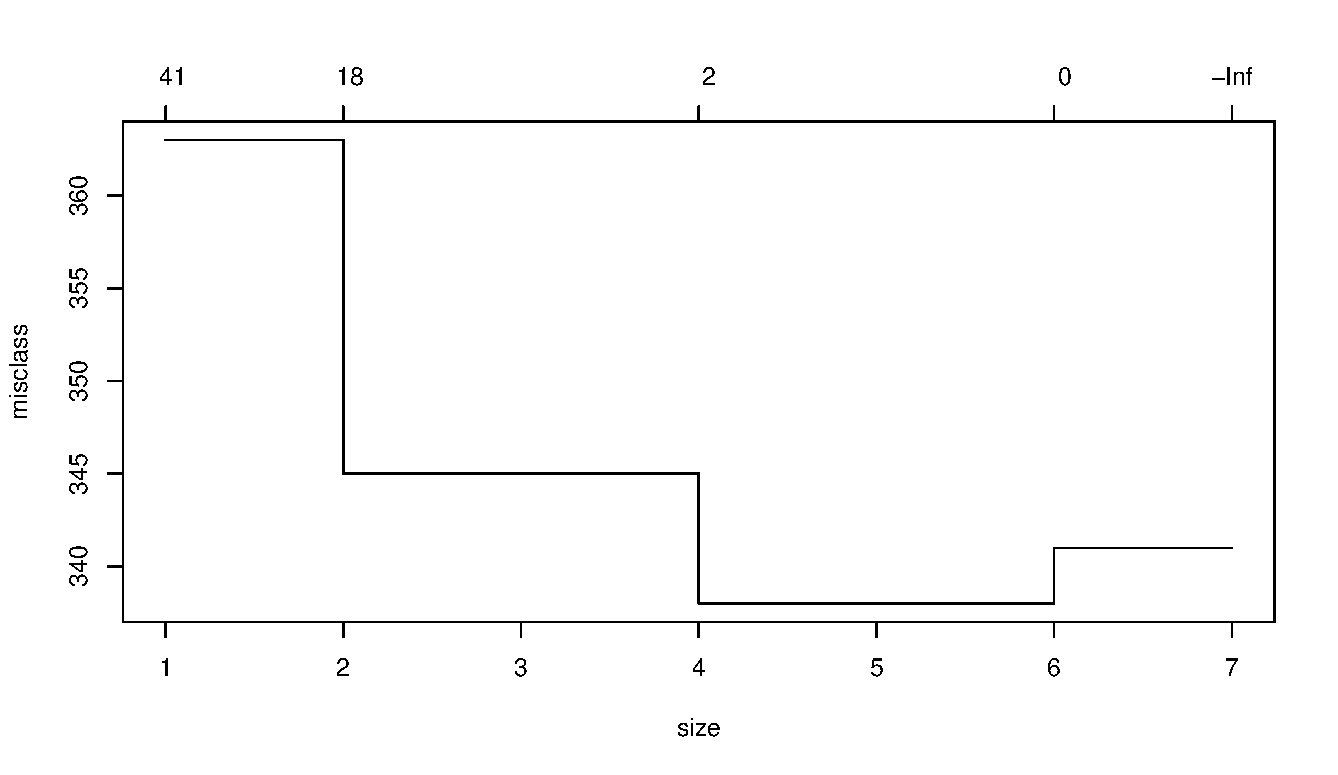
\includegraphics[width=0.5\linewidth]{ImageFiles/Classification/Trees/tree_cv_plot.pdf}
	\caption{Size (bottom), deviance (left), k (top).}
	\label{fig:tree_cv_plot}
\end{figure}

\begin{figure}[H]
	\centering
	\begin{subfigure}{.5\textwidth}
		\centering
		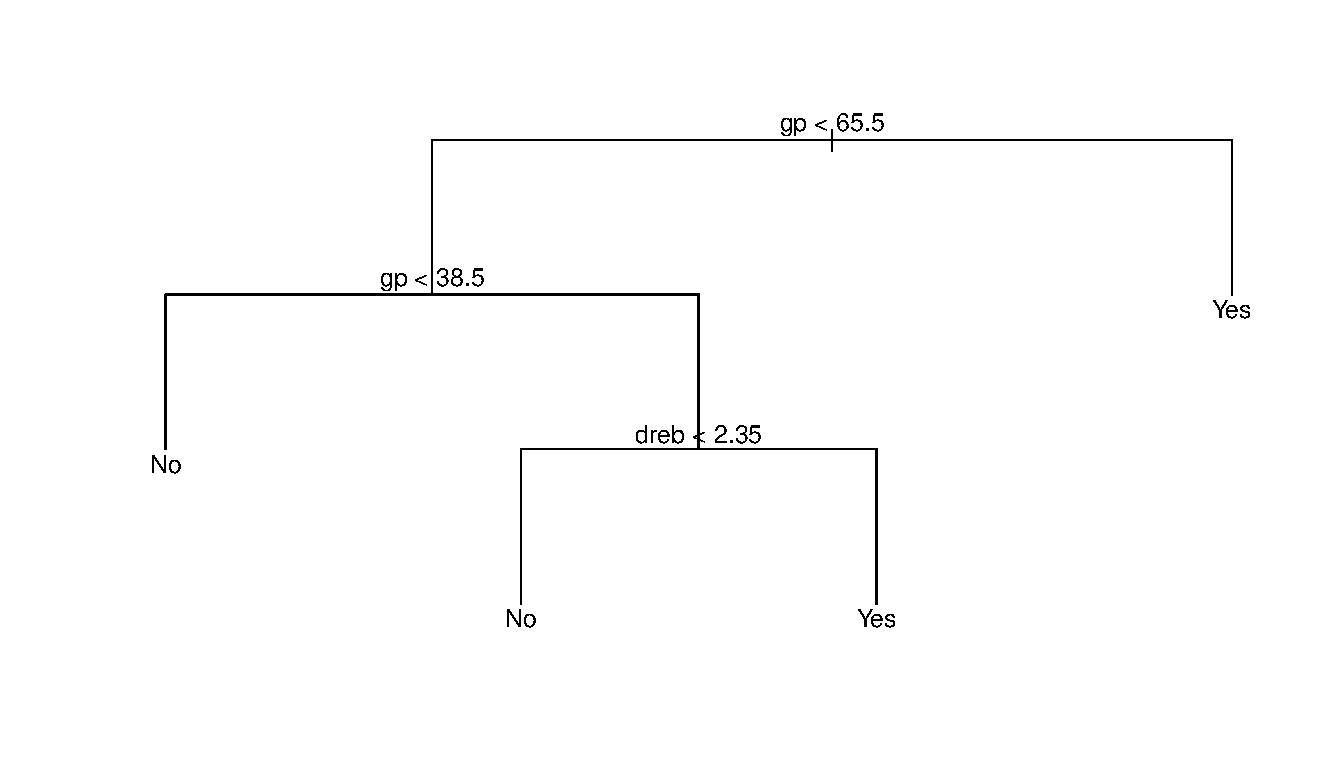
\includegraphics[width=0.6\linewidth]{ImageFiles/Classification/Trees/tree_size_4.pdf}
		\caption{}
		\label{fig:tree_size_4}
	\end{subfigure}%
	\begin{subfigure}{.5\textwidth}
		\centering
		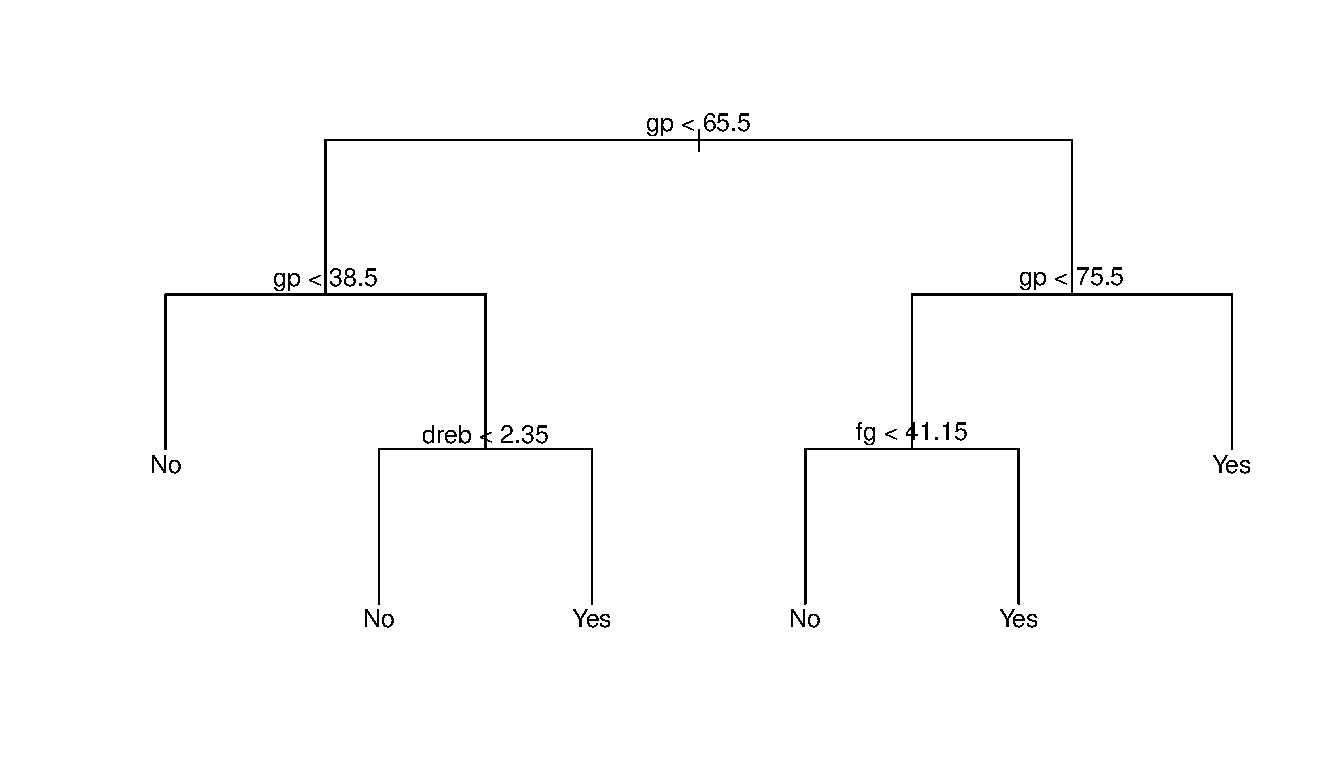
\includegraphics[width=0.6\linewidth]{ImageFiles/Classification/Trees/tree_size_6.pdf}
		\caption{}
		\label{fig:tree_size_6}
	\end{subfigure}
	\begin{subfigure}{.5\textwidth}
		\centering
		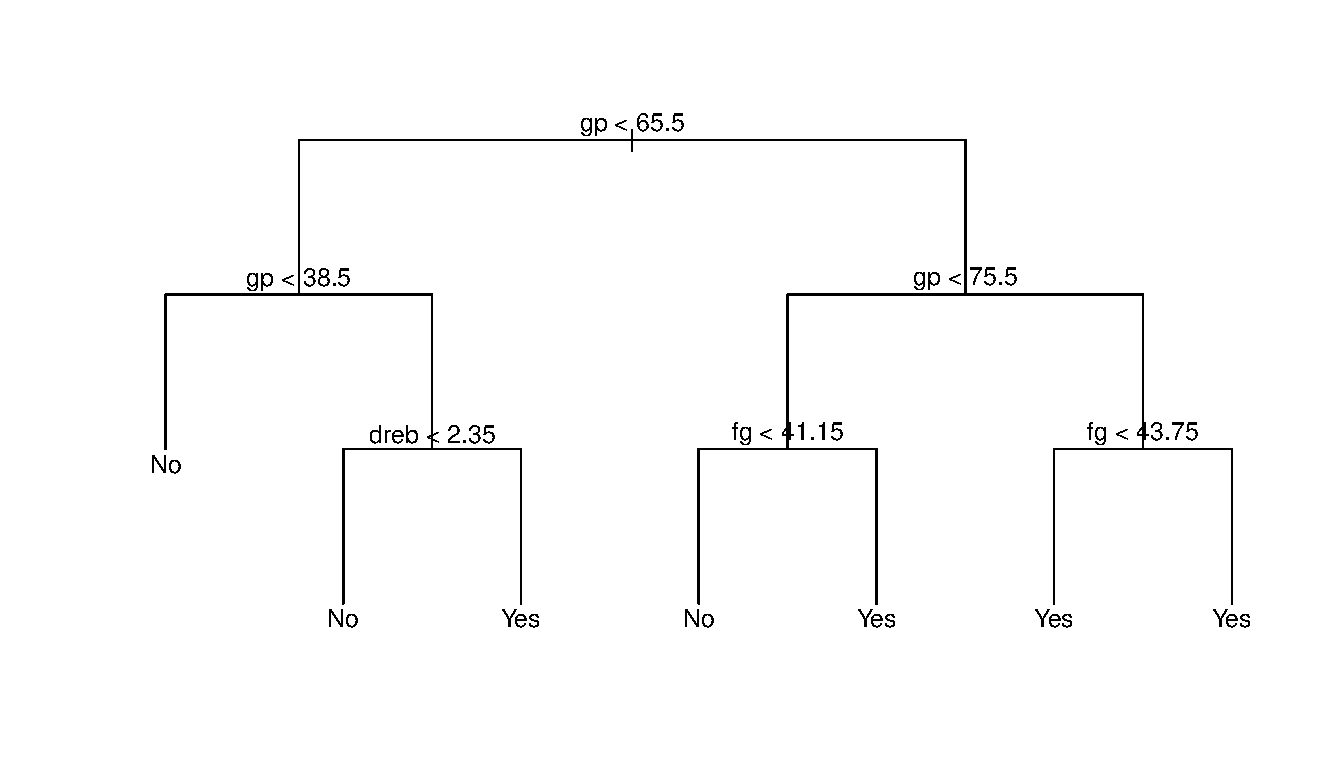
\includegraphics[width=0.6\linewidth]{ImageFiles/Classification/Trees/tree_size_7.pdf}
		\caption{}
		\label{fig:tree_size_7}
	\end{subfigure}%
	\begin{subfigure}{.5\textwidth}
		\centering
		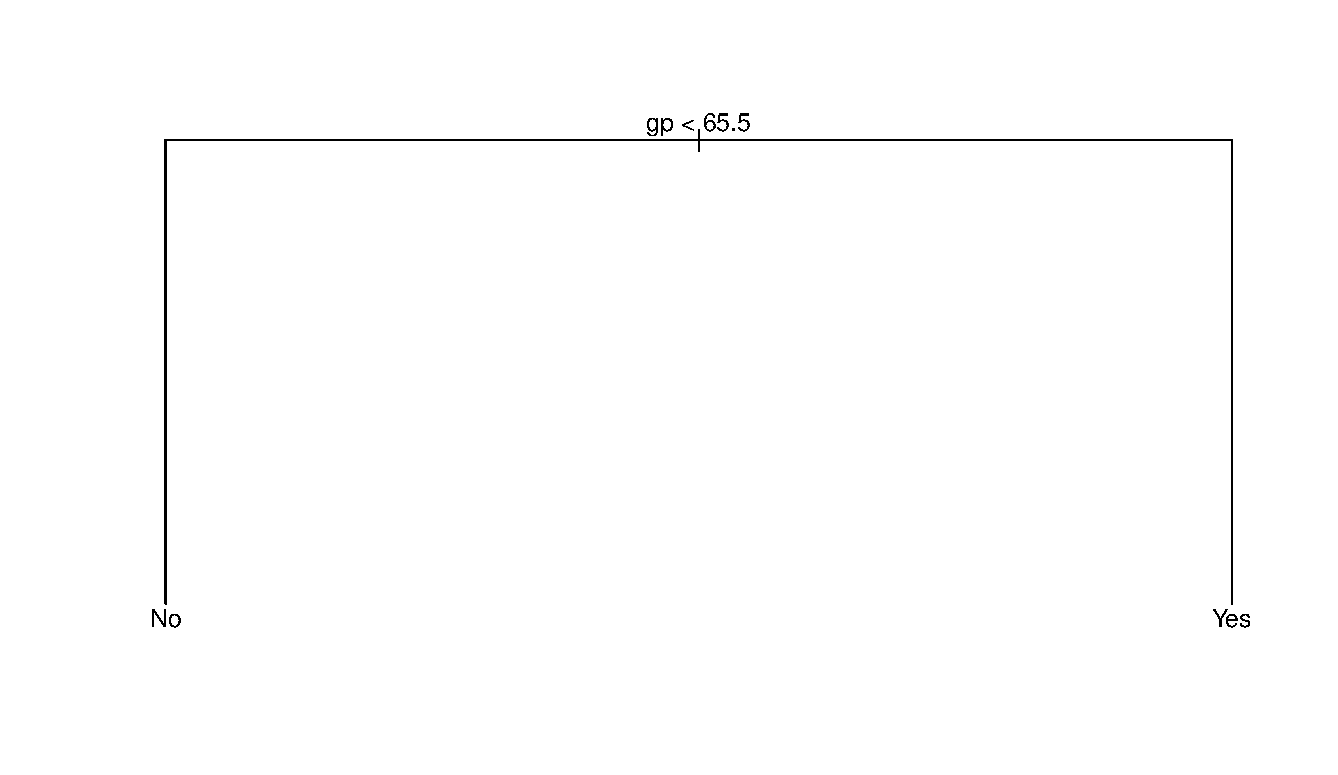
\includegraphics[width=0.6\linewidth]{ImageFiles/Classification/Trees/tree_size_2.pdf}
		\caption{}
		\label{fig:tree_size_2}
	\end{subfigure}
	\caption{Trees with various sizes. (a)4. (b)6. (c)7. (d)2.}
	\label{fig:trees_size}
\end{figure}

After the evaluation of the MER on both train and test dataset, we concluded that the best model is the one with $size = 4$.

\begin{table}[H]
	\centering
	\begin{tabular}{|| c | c | c ||}
		\hline 
		Tree size & MER\_train(\%) & MER\_test(\%) \\
		\hline
		109 & 0.2067 & 0.3469 \\
		\hline
		4 & 0.3038 & 0.3000 \\
		\hline
		6 & 0.2996 & 0.33125 \\
		\hline
		7 & 0.2996 & 0.33125 \\
		\hline
		2 & 0.3424 & 0.33125 \\
		\hline
	\end{tabular}
	\caption{Different tree size results.}
\end{table} 

Nonetheless, the variable ``GP'' consistently serves as the first split in all the trees, indicating its significance as the most important variable. Although ``DREB'' and ``FG\%'' also appear in splits within larger-sized trees, "GP" continues to be the variable that undergoes the highest number of splits.

Despite ``GP'' being a positive integer variable, it is noteworthy that the splits on ``GP'' consistently happen at decimal values (e.g., 65.5 in the first split of all trees). This occurrence arises because the trees aim to divide the samples into two classes, distinguishing samples with ``GP'' values greater than or equal to 66 from those with ``GP'' values less than or equal to 65.
